% ★★★ 难题
\newcommand{\qSolidTrianglesFoldingStem}{
现有两块含 \(30^\circ\) 角的全等直角三角板，较短直角边长均为 \(10\,\mathrm{cm}\)。

如图，\(\triangle PAB\) 与 \(\triangle PCD\) 为这两块三角板，其中
\[
PA=PC=10\,\mathrm{cm}, \qquad \angle PBA=\angle PDC=30^\circ.
\]
初始时，将这两块三角板的直角顶点重合于点 \(P\)，斜边 \(AB\)、\(CD\) 共线，如图~1 所示。
然后将这两块三角板分别绕点 \(P\) 向相反方向转动，得到四棱锥 \(P-ABCD\)，如图~2 所示。

\begin{enumerate}
    \item 求证：平面 \(PAC\perp\) 平面 \(ABCD\)。
    \item 设平面 \(PAB\cap\) 平面 \(PCD=l\)。
    \begin{enumerate}
        \item[(i)] 求直线 \(l\) 与直线 \(PA\) 所成角的大小；
        \item[(ii)] 当二面角 \(A-l-C\) 的大小为 \(\frac{\pi}{3}\) 时，求四棱锥 \(P-ABCD\) 的体积。
    \end{enumerate}
\end{enumerate}
}

\newcommand{\qSolidTrianglesFoldingFigure}[1][1.0]{
    \centering
    %====================== 图1 ======================%
    \begin{minipage}[c]{0.48\textwidth}
        \centering
        \begin{tikzpicture}[
            scale=1.2*#1,
            line cap=round,
            line join=round,
            every node/.style={font=\small}
        ]
        \coordinate (P) at (0, 1.732);
        \coordinate (B) at (-3, 0);
        \coordinate (C) at (-1, 0);
        \coordinate (A) at (1, 0);
        \coordinate (D) at (3, 0);

        \draw[thick] (B)--(D);
        \draw[thick] (P)--(B);
        \draw[thick] (P)--(C);
        \draw[thick] (P)--(A);
        \draw[thick] (P)--(D);

        \pic[
            draw,
            "$30^\circ$",
            angle radius=7mm,
            angle eccentricity=1.45
        ] {angle=A--B--P};

        \pic[
            draw,
            "$30^\circ$",
            angle radius=7mm,
            angle eccentricity=1.45
        ] {angle=P--D--C};

        \coordinate (PA1) at ($(P)!3mm!(A)$);
        \coordinate (PB1) at ($(P)!3mm!(B)$);
        \draw (PA1) -- ($(PA1)+(PB1)-(P)$) -- (PB1);

        \coordinate (PC1) at ($(P)!3mm!(C)$);
        \coordinate (PD1) at ($(P)!3mm!(D)$);
        \draw (PC1) -- ($(PC1)+(PD1)-(P)$) -- (PC1);

        \fill (P) circle (1pt);
        \fill (B) circle (1pt);
        \fill (C) circle (1pt);
        \fill (A) circle (1pt);
        \fill (D) circle (1pt);

        \node[above]       at (P) {$P$};
        \node[below left]  at (B) {$B$};
        \node[below]       at (C) {$C$};
        \node[below]       at (A) {$A$};
        \node[below right] at (D) {$D$};
        \end{tikzpicture}
        \par\vspace{0.3em}{\small 图 1}
    \end{minipage}
    \hfill
    %====================== 图2 ======================%
    \begin{minipage}[c]{0.48\textwidth}
        \centering
        \begin{tikzpicture}[
            scale=1.2*#1,
            line cap=round,
            line join=round,
            every node/.style={font=\small},
            x={(1cm,0cm)}, y={(0.5cm,0.35cm)}, z={(0cm,1cm)}
        ]
        \coordinate (P) at (0, 0, 1.5);
        \coordinate (A) at (1, 0.866, 0);
        \coordinate (B) at (-3, 0.866, 0);
        \coordinate (C) at (-1, -0.866, 0);
        \coordinate (D) at (3, -0.866, 0);

        \pic[
            draw,
            "$30^\circ$",
            angle radius=7mm,
            angle eccentricity=1.4,
            font=\footnotesize
        ] {angle=A--B--P};

        \pic[
            draw,
            "$30^\circ$",
            angle radius=7mm,
            angle eccentricity=1.4,
            font=\footnotesize
        ] {angle=P--D--C};

        \draw[thick] (B)--(C)--(D);
        \draw[thick,dashed] (D)--(A)--(B);

        \draw[thick] (P)--(B);
        \draw[thick] (P)--(C);
        \draw[thick] (P)--(D);
        \draw[thick,dashed] (P)--(A);

        \coordinate (PA2) at ($(P)!3mm!(A)$);
        \coordinate (PB2) at ($(P)!3mm!(B)$);
        \draw[dashed] (PA2) -- ($(PA2)+(PB2)-(P)$) -- (PB2);

        \coordinate (PC2) at ($(P)!3mm!(C)$);
        \coordinate (PD2) at ($(P)!3mm!(D)$);
        \draw (PC2) -- ($(PC2)+(PD2)-(P)$) -- (PD2);

        \draw[thick, dash dot] (-2.5, 0, 1.5) -- (2.5, 0, 1.5) node[right] {$l$};

        \fill (P) circle (1pt);
        \fill (A) circle (1pt);
        \fill (B) circle (1pt);
        \fill (C) circle (1pt);
        \fill (D) circle (1pt);

        \node[above]       at (P) {$P$};
        \node[above right] at (A) {$A$};
        \node[left]        at (B) {$B$};
        \node[below]       at (C) {$C$};
        \node[right]       at (D) {$D$};
        \end{tikzpicture}
        \par\vspace{0.3em}{\small 图 2}
    \end{minipage}
}

\newcommand{\qSolidTrianglesFoldingAnswer}{
(1) 证明见解析；(2)(i) 直线 \(l\) 与直线 \(PA\) 所成角为 \(60^\circ\)；(ii) 四棱锥 \(P-ABCD\) 的体积为 \(250\sqrt{3}\)。
}

\newcommand{\qSolidTrianglesFoldingSolution}{
\subsection*{（1）证明：平面 $PAC \perp$ 平面 $ABCD$}
设点 $P$ 在平面 $ABCD$ 上的投影为 $O$，连接 $OA, OB, OC, OD$。
因为 $PO \perp$ 平面 $ABCD$，根据勾股定理有：
\[
OA = \sqrt{PA^2 - PO^2}, \quad OC = \sqrt{PC^2 - PO^2}
\]
由题意 $PA = PC = 10$，可得 $OA = OC$。
同理，因为 $PB = PD = 10\sqrt{3}$，可得 $OB = OD$。

结合题意与空间几何的对称性可知，在转动过程中 $AB$ 与 $CD$ 始终保持平行。
因为 $AB \parallel CD$ 且 $AB = CD = 20$，所以底面 $ABCD$ 必然是平行四边形。
在平行四边形 $ABCD$ 中，到相对顶点距离相等的点 $O$ 必然是它的对角线交点（中心）。
因此，点 $O$ 位于对角线 $AC$ 上。
由于 $PO \perp$ 平面 $ABCD$，且 $PO \subset$ 平面 $PAC$，
根据面面垂直的判定定理，可得 平面 $PAC \perp$ 平面 $ABCD$。

\begin{center}
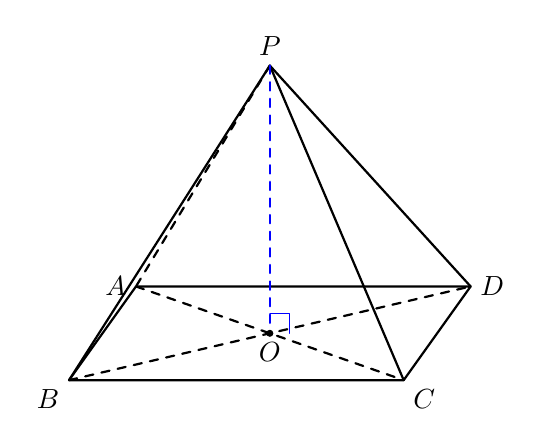
\begin{tikzpicture}[
    scale=0.85,
    line cap=round,
    line join=round,
    x={(1cm,0cm)}, y={(0.5cm,0.35cm)}, z={(0cm,1cm)}
]
\coordinate (O) at (0,0,0);
\coordinate (P) at (0,0,4);
\coordinate (A) at (-3, 2, 0);
\coordinate (B) at (-2, -2, 0);
\coordinate (C) at (3, -2, 0);
\coordinate (D) at (2, 2, 0);

\draw[thick] (A)--(B)--(C)--(D)--cycle;
\draw[thick] (P)--(B);
\draw[thick] (P)--(C);
\draw[thick] (P)--(D);
\draw[thick, dashed] (P)--(A);
\draw[thick, dashed] (A)--(C);
\draw[thick, dashed] (B)--(D);
\draw[thick, dashed, blue] (P)--(O);

\fill (O) circle (1.5pt) node[below] {$O$};
\node[above] at (P) {$P$};
\node[left]  at (A) {$A$};
\node[below left]  at (B) {$B$};
\node[below right] at (C) {$C$};
\node[right] at (D) {$D$};

\coordinate (O1) at (0.3, 0, 0);
\coordinate (O2) at (0.3, 0, 0.3);
\coordinate (O3) at (0, 0, 0.3);
\draw[blue] (O1) -- (O2) -- (O3);
\end{tikzpicture}
\par\vspace{0.3em}{\small 图 3：投影 $O$ 与四棱锥的高}
\end{center}

\subsection*{（2）解：}
\textbf{(i) 直线 $l$ 与直线 $PA$ 所成角}

因为 平面 $PAB \cap$ 平面 $PCD = l$，
且在平行四边形 $ABCD$ 中有 $AB \parallel CD$。
又 $AB \subset$ 平面 $PAB$，$CD \subset$ 平面 $PCD$，
根据线面平行的性质定理，可知 $l \parallel AB$（且 $l \parallel CD$）。
所以直线 $l$ 与直线 $PA$ 所成的角，即为 $AB$ 与 $PA$ 所成的角（即 $\angle PAB$）。

在 $\mathrm{Rt}\triangle PAB$ 中，$\angle APB = 90^\circ, \angle PBA = 30^\circ$，
所以 $\angle PAB = 60^\circ$。
即直线 $l$ 与直线 $PA$ 所成角的大小为 $60^\circ$（或 $\frac{\pi}{3}$）。

\textbf{(ii) 四棱锥 $P-ABCD$ 的体积}

在 $\triangle PAB$ 与 $\triangle PCD$ 中，分别作 $PE \perp AB$ 于 $E$，$PF \perp CD$ 于 $F$。
因为 $PA=10, PB=10\sqrt{3}, AB=20$，利用等面积法求得高：
\[
PE = \frac{PA \cdot PB}{AB} = 5\sqrt{3}
\]
同理 $PF = 5\sqrt{3}$。

由于 $l \parallel AB$ 且 $l \parallel CD$，ので $PE \perp l$ 且 $PF \perp l$。
因此，$\angle EPF$ 即为二面角 $A-l-C$ 的平面角。
由题意，二面角大小为 $\frac{\pi}{3}$，即 $\angle EPF = 60^\circ$。
在 $\triangle EPF$ 中，$PE = PF = 5\sqrt{3}$，且 $\angle EPF = 60^\circ$，
所以 $\triangle EPF$ 是边长为 $5\sqrt{3}$ 的等边三角形，故 $EF = 5\sqrt{3}$。

\begin{center}
\begin{tikzpicture}[
    scale=0.85,
    line cap=round,
    line join=round,
    every node/.style={font=\small},
    x={(1cm,0cm)}, y={(0.5cm,0.35cm)}, z={(0cm,1cm)}
]
\coordinate (P) at (0, 0, 0);
\draw[thin] (-4.5, 0, 0) -- (4.5, 0, 0) -- (6.0, 2.5, 0) -- (-3.0, 2.5, 0) -- cycle;
\node[below left] at (6.0, 2.5, 0) {$\beta$};

\draw[thin] (-4.5, 0, 0) -- (4.5, 0, 0) -- (6.0, 1.25, 2.165) -- (-3.0, 1.25, 2.165) -- cycle;
\node[below left] at (6.0, 1.25, 2.165) {$\alpha$};

\draw[thick, dash dot] (-5.5, 0, 0) -- (5.5, 0, 0) node[right] {$l$};

\coordinate (F) at (0, 1.732, 0);
\coordinate (C) at (-1, 1.732, 0);
\coordinate (D) at (3, 1.732, 0);

\coordinate (E) at (0, 0.866, 1.5);
\coordinate (A) at (1, 0.866, 1.5);
\coordinate (B) at (-3, 0.866, 1.5);

\draw[thick, dashed] (A)--(D);
\draw[thick, dashed] (B)--(C);

\draw[thick] (A)--(B);
\draw[thick] (C)--(D);
\draw[thick] (P)--(A);
\draw[thick] (P)--(B);
\draw[thick] (P)--(C);
\draw[thick] (P)--(D);

\draw[thick, dashed, blue] (P)--(E);
\draw[thick, dashed, blue] (P)--(F);

\coordinate (EA) at ($(E)!3mm!(A)$);
\coordinate (EP) at ($(E)!3mm!(P)$);
\draw (EA) -- ($(EA)+(EP)-(E)$) -- (EP);

\coordinate (FD) at ($(F)!3mm!(D)$);
\coordinate (FP) at ($(F)!3mm!(P)$);
\draw (FD) -- ($(FD)+(FP)-(F)$) -- (FP);

\pic[
    draw, blue,
    "$\frac{\pi}{3}$",
    angle radius=8mm,
    angle eccentricity=1.3
] {angle=F--P--E};

\node[below] at (P) {$P$};
\node[above] at (A) {$A$};
\node[above] at (B) {$B$};
\node[left]  at (C) {$C$};
\node[right] at (D) {$D$};
\node[above right] at (E) {$E$};
\node[below right] at (F) {$F$};
\end{tikzpicture}
\par\vspace{0.3em}{\small 图 4：二面角 $A-l-C$ 与辅助面}
\end{center}

由（1）可知，$P$ 在底面的投影 $O$ 是平行四边形的中心。
根据三垂线定理的逆定理，因为 $PO \perp$ 平面 $ABCD$ 且 $PE \perp AB$，可得 $OE \perp AB$；同理 $OF \perp CD$。
因为 $AB \parallel CD$，所以 $E, O, F$ 三点共线，线段 $EF$ 的长度即为平行四边形 $ABCD$ 两平行边 $AB, CD$ 之间的距离。
所以底面 $ABCD$ 的面积为：
\[
S_{ABCD} = AB \cdot EF = 20 \times 5\sqrt{3} = 100\sqrt{3}
\]

在等边 $\triangle EPF$ 中，$PO$ 为边 $EF$ 上的高，
所以四棱锥的高为：
\[
h = PO = PE \cdot \sin 60^\circ = 5\sqrt{3} \times \frac{\sqrt{3}}{2} = \frac{15}{2}
\]

故四棱锥 $P-ABCD$ 的体积为：
\[
V = \frac{1}{3} S_{ABCD} \cdot h = \frac{1}{3} \times 100\sqrt{3} \times \frac{15}{2} = 250\sqrt{3}
\]

\subsection*{方法二：空间向量分解法（基底法）}
我们在解决二面角和体积计算时，还可以利用交线 $l$ 及其垂线方向作为基底进行向量分解。

\textbf{(i) 直线 $l$ 与直线 $PA$ 所成角}

由题意，平面 $PAB \cap$ 平面 $PCD = l$。因为在四棱锥底面中 $AB \parallel CD$，由线面平行的性质定理可知 $l \parallel AB$。
设单位向量 $\vec{e}$ 的方向与 $\overrightarrow{AB}$ 相同。
在 $\triangle PAB$ 中作 $PE \perp AB$ 于 $E$。根据向量的加法法则，有：
\[ \overrightarrow{PA} = \overrightarrow{PE} + \overrightarrow{EA} \]
因为 $PE \perp AB$，所以 $\overrightarrow{PE} \cdot \vec{e} = 0$。
由于 $\overrightarrow{EA}$ 与 $\vec{e}$ 共线，结合 $\mathrm{Rt}\triangle PAB$ 的边长关系（$PA=10, PB=10\sqrt{3}, AB=20$），可求得投影 $AE = 5, PE = 5\sqrt{3}$。
因为 $\overrightarrow{EA}$ 的方向与 $\overrightarrow{AB}$ 相反，所以 $\overrightarrow{EA} \cdot \vec{e} = -5$。
则向量 $\overrightarrow{PA}$ 与 $l$ 方向单位向量 $\vec{e}$ 的数量积为：
\[ \overrightarrow{PA} \cdot \vec{e} = (\overrightarrow{PE} + \overrightarrow{EA}) \cdot \vec{e} = 0 - 5 = -5 \]
设 $\overrightarrow{PA}$ 与 $\vec{e}$ 的夹角为 $\alpha$，则：
\[ \cos \alpha = \frac{\overrightarrow{PA} \cdot \vec{e}}{|\overrightarrow{PA}| |\vec{e}|} = \frac{-5}{10 \times 1} = -\frac{1}{2} \]
故直线 $l$ 与直线 $PA$ 所成角为 $60^\circ$。

\textbf{(ii) 四棱锥 $P-ABCD$ 的体积}

在 $\triangle PCD$ 中同理作 $PF \perp CD$ 于 $F$，可得 $PF = 5\sqrt{3}$。
因为 $l \parallel AB \parallel CD$ 且 $PE \perp AB, PF \perp CD$，所以 $PE \perp l$ 且 $PF \perp l$。
这说明向量 $\overrightarrow{PE}$ 与 $\overrightarrow{PF}$ 的夹角即为二面角 $A-l-C$ 的平面角，即 $\langle \overrightarrow{PE}, \overrightarrow{PF} \rangle = 60^\circ$。

选取不共面的向量 $\{\overrightarrow{PE}, \overrightarrow{PF}, \vec{e}\}$ 作为基底。
设点 $O$ 为线段 $EF$ 的中点，则 $\overrightarrow{PO} = \frac{1}{2}(\overrightarrow{PE} + \overrightarrow{PF})$。
我们来验证 $PO$ 是否为四棱锥的高。
首先计算 $\overrightarrow{PO} \cdot \overrightarrow{EF}$：
\[
\overrightarrow{PO} \cdot \overrightarrow{EF} = \frac{1}{2}(\overrightarrow{PE} + \overrightarrow{PF}) \cdot (\overrightarrow{PF} - \overrightarrow{PE}) = \frac{1}{2}(|\overrightarrow{PF}|^2 - |\overrightarrow{PE}|^2) = \frac{1}{2}(75 - 75) = 0
\]
so $PO \perp EF$。
再计算 $\overrightarrow{PO} \cdot \vec{e}$：
\[
\overrightarrow{PO} \cdot \vec{e} = \frac{1}{2}(\overrightarrow{PE} \cdot \vec{e} + \overrightarrow{PF} \cdot \vec{e}) = \frac{1}{2}(0 + 0) = 0
\]
所以 $PO \perp l$（即 $PO \perp AB$）。
由于 $PO$ 垂直于底面内两条相交直线 $EF$ 和 $AB$，故 $PO \perp$ 平面 $ABCD$，即 $PO$ 就是四棱锥的高 $h$。

利用数量积的性质直接求高 $h = |\overrightarrow{PO}|$：
\[
h^2 = |\overrightarrow{PO}|^2 = \frac{1}{4}(\overrightarrow{PE} + \overrightarrow{PF})^2 = \frac{1}{4}\left(|\overrightarrow{PE}|^2 + |\overrightarrow{PF}|^2 + 2|\overrightarrow{PE}||\overrightarrow{PF}|\cos 60^\circ\right)
\]
\[
h^2 = \frac{1}{4}\left(75 + 75 + 2 \times 75 \times \frac{1}{2}\right) = \frac{225}{4} \implies h = \frac{15}{2}
\]

同时，底面平行四边形的高（即平行线 $AB$ 与 $CD$ 的距离）就是线段 $EF$ 的长度：
\[
EF^2 = |\overrightarrow{PF} - \overrightarrow{PE}|^2 = |\overrightarrow{PE}|^2 + |\overrightarrow{PF}|^2 - 2|\overrightarrow{PE}||\overrightarrow{PF}|\cos 60^\circ = 75 + 75 - 75 = 75 \implies EF = 5\sqrt{3}
\]
底面积 $S_{ABCD} = AB \cdot EF = 20 \times 5\sqrt{3} = 100\sqrt{3}$。
所以四棱锥体积为：
\[
V = \frac{1}{3} S_{ABCD} \cdot h = \frac{1}{3} \times 100\sqrt{3} \times \frac{15}{2} = 250\sqrt{3}
\]
}
